
% JuliaCon proceedings template
\documentclass{juliacon}
\usepackage{minted}
\setcounter{page}{1}

\begin{document}

% **************GENERATED FILE, DO NOT EDIT**************

\title{Lyapunov Cycle Detector (LCD.jl): A new tool for the study of basins of attraction induced by rational maps}

\author[1]{V. Álvarez-Aparicio}
\affil[1]{University of La Rioja, Spain}

\keywords{Cycles, Julia sets, Basins of attraction, Dynamical Systems, Lyapunov exponents, Rational maps, Numerical Analysis, Complex Dynamics, Julia Language, Parallel programming}

\maketitle

\textit{Summary}. We present Lyapunov Cycle Detector (LCD.jl), a package that provides useful tools to study and visualize the basins of attraction induced by a complex rational map. The algorithms implemented in it utilize Hopf-endomorphisms and Lyapunov exponents to compute and distinguish the basins of attraction. Also, they benefit from the estructure of the complex projective line $P^1(\mathbb{C})$ in order to avoid numerical overflows and indeterminations, and use some of Julia's built-in multi-threading features, reducing significantly the execution time of the algorithms.\\

\textit{Presentation}. To describe and compute the basins of attraction induced by a complex rational map has traditionally been a very relevant matter in the study of certain branches of Mathematics, such as Numerical Analysis, Complex Dynamics or Discrete-time Dynamical Systems. From a computational perspective, when performing this calculations, some numerical problems as overflows, underflows or indeterminations might arise and affect the obtained results. In addition, approximating the basins of attraction often has a significant computational cost, depending on the parameters and precision considered.

In the Lyapunov Cycle Detector (LCD.jl) package \cite{alvarez}, we include the implementation in Julia Language \cite{bezanson} of the methods described by the authors in \cite{preprint}, where one can find the proofs and the mathematical background that support these algorithms. They have been developed according to several goals, among which we highlight the following:
\begin{enumerate}
    \item Being able to avoid indeterminations, overflows, underflows and other computational problems that often appear in software devoted to Numerical Analysis.
    \item Consider the infinity point and work comfortably with it.
    \item Achieve a fast and efficient execution of the algorithms.
    \item In addition to computing the basins of attraction, extract some useful information about the discrete-time dynamical system induced by the iteration of the rational map.
\end{enumerate}
Thanks to this approach, the benefits that this newly implemented algorithms provide have lead to better results both numerically (avoiding the previously mentioned computational problems) and computationally (in terms of efficiency and execution time) in comparison with other algorithms that have been developed by the authors, see \cite{julia}, \cite{lj}, \cite{sage}.\\

\textit{Usage}. In the Lyapunov Cycle Detector repository one can find multiple methods for many different purposes, such as iterating the Hopf-endomorphism associated to a given rational map or approximating the Lyapunov function described in \cite{preprint}. However, the main functionality of this package is to compute and visualize the basins of attraction of a complex rational map. This can be achieved through the following method:
\begin{minted}{julia}
gra=LCD.plotBasinsOfAttraction_Lyapunov(coefnum,
    coefden,(-1.5,1.5),(-1.5,1.5),200,1,8;
    coloringStrat="position",inverted=false)
img=gra[1]
numColors=gra[2]
\end{minted}
where \textit{coefnum} and \textit{coefden} contain the coefficients of the numerator and denominator of the rational map respectively, the considered region of the complex plane $\mathbb{C}$ is $(-1.5,1.5)\times(-1.5,1.5)$, $200$ is the maximum number of iterations allowed, $1$ is the maximum length of the $n$-cycles we want to compute, $8$ corresponds to the considered tolerance ($10^{-8}$), and \textit{coloringStrat} and \textit{inverted} determine how the basins are visualized.

In the two previous images we can see the resulting graphs of this method, considering \textit{inverted} as \textit{false} or \textit{true} respectively.

\begin{figure}
\begin{center}
    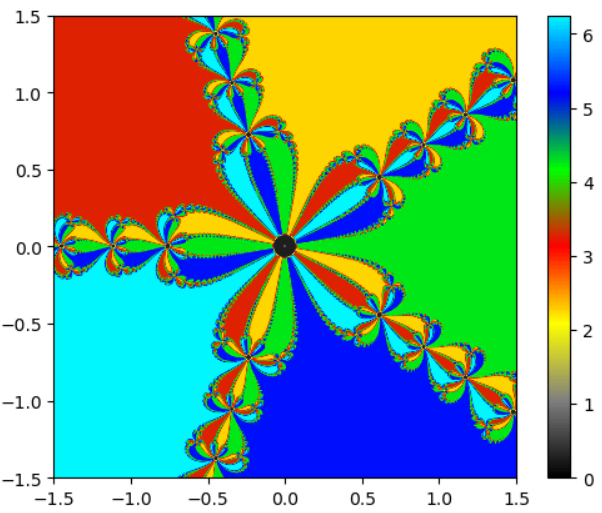
\includegraphics[width=5.5cm]{z^5-1_(origin).PNG}
\end{center}
\end{figure}
\begin{figure}
\begin{center}
    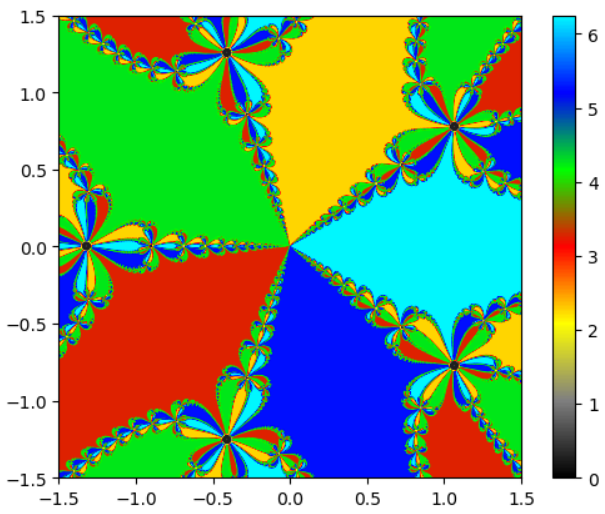
\includegraphics[width=5.5cm]{z^5-1_(infinity).PNG}
\end{center}
\end{figure}


% **************GENERATED FILE, DO NOT EDIT**************

\bibliographystyle{juliacon}
\bibliography{ref.bib}

\end{document}

% Inspired by the International Journal of Computer Applications template